\section{User Interface Entwürfe}

Die User Interfaces wurden so gestaltet, dass sie die zuvor genannten User Stories, Use Cases und Anforderungen bestmöglich erfüllen. 
\paragraph{}Dabei werden die Mitarbeiter Use Cases in einer mobile first Anwendung verpackt, weil die Arbeitsplatzbuchungen schnell und leicht von der Hand gehen sollen.
Ebenfalls ist mobile first praktisch für die Nachtrichten-Funktion, da die Erreichbarkeit und die Möglichkeit schnell zu antworten, auf mobilen Geräten besser ist als auf Desktop Systemen. 
\paragraph{}Die Use Cases des Administrators und der Geschäftsführung werden wiederum auf Desktop-Systeme ausgelegt, da dort eine übersichtliche, effiziente und präzise Nutzung wichtiger ist, als die Flexibilität auf das System zuzugreifen zu können. 

\subsection{Mitarbeiter User Interface}

Nachfolgend werden die Funktionen und Seiten des mobile first User Interfaces visualisiert und erläutert. 

\subsubsection{Buchen}

\begin{wrapfigure}{r}{5.5cm}
    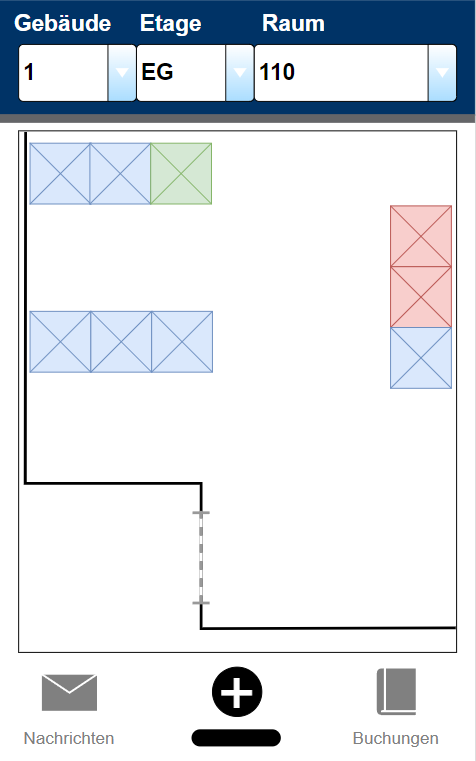
\includegraphics[width=4.5cm]{sketchBooking.png}
    \caption{User Interface: Buchen}
  \end{wrapfigure}

Sobald die Anwendung abgerufen wird, erhält man das Buchen-Fenster.
\paragraph{}Ersichtlich ist das aktuell geöffnete Fenster durch die Funktionsleiste am unteren Ende der Anwendung. 
Dort wird die ausgewählte Funktion, spricht das aktuelle Fenster, durch die dunkel schwarze Färbung und den Balken darunter hervorgehoben.
\paragraph{}Im oberen Teil der Anwendung kann man über Dropdown-Menus sich das Gebäude, die Etage und den Raum raussuchen, in dem mach buchen möchte.
Dabei wählt man von rechts startend aus, spricht zuerst das Gebäude, dann die Etage und zuletzt den Raum.
Dies ist wichtig, weil je nach Gebäude andere Etagen bestehen, welche dann wieder nur bestimmte Räume enthalten.

\paragraph{}Wenn im oberen Teil alle Angaben bis zum Raum hin gegeben wurden, sieht man in der Mitte der Anwendung den ausgewählten Raum.
Dieser wird durch ein Rechteck mit dünnen  schwarzen Linien in der Anwendung begrenzt.
In diesem Rahmen soll es möglich sein den Raum zu verschieben und zu vergrößern und zu verkleinern.
Der Raum an sich besteht zum einen aus Wänden, dicke schwarze Striche, und Türen, grau gestrichelte Einsätze in den Wänden. Türen und Wände werden 
lediglich zur Orientierung und besseren Vorstellung des Raumes genutzt. 
\paragraph{}In dem Raum befinden sich schließlich farbige Rechtecke, welche Arbeitsplätze darstellen, mit denen man interagieren kann. Die farbliche Kennzeichnung beschreibt, wie der Platz an dem heutigen Tag genutzt wird.
Blau zeigt an, dass der Platz frei verfügbar ist für heute, rot zeigt an, dass der Platz mindestens in einem Zeitfenster von heute eine Buchung eines anderen Arbeitskollegen vorliegen hat und grün zeigt an, dass man den Arbeitsplatz für heute selbst in mindestens einem Zeitfenster gebucht hat.
\paragraph{}Um weitere und genauere Informationen über die Belegung eines Arbeitsplatzes zu erhalten, klickt man diesen an.

\begin{wrapfigure}{r}{5.5cm}
  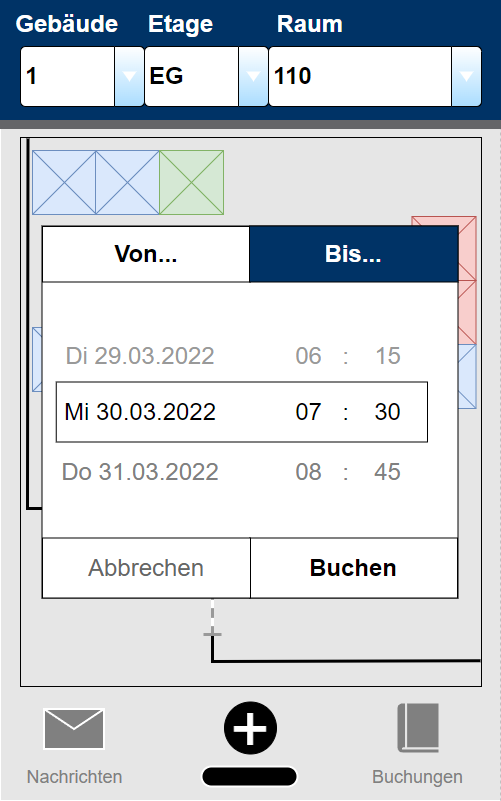
\includegraphics[width=4.5cm]{sketchTime1.png}
  \caption{User Interface: Buchen - Zeitauswahl}
\end{wrapfigure}

\paragraph{}Mit dem Anklicken erscheint ein Pop-Up Fenster, für die Zeiteingabe. 
In der Mitte des Fensters befindet sich die Zeitanagebe, die man aktuell ausgewählt hat. 
Durch unabhängiges hoch- und runterswipen des Datums, der Stunden und Minuten verändert man die Zeitangabe.
Die Zeitangaben sind dabei in 15-Minutenschlitze unterteilt.

\paragraph{} Zu Beginn startet man mit der "`Von"' Zeitangabe, welche den Start des Buchungszeitraumes festlegt. 
Im oberen Teil des Pop-Ups wird durch blaue Farbe hervorgehoben, ob es sich um die Eingabe der Startzeit oder der Endzeit handelt.
Mit einem Klick auf "`Von..."' oder "`Bis..."' lassen sich somit auch die zeiteingaben dafür wechseln. 

\paragraph{}Im unteren Teil des Pop-Ups kann man sets die Eingaben verwerfen durch einen Klick auf "Abbrechen".
Rechts daneben kann man die Eingaben bestätigen und abschicken durch einen Klick auf "`Buchen"'.
Dabei ist der Buchen-Button bei nur einer "`Von"' Angabe noch ausgegraut und nicht anklickbar.
Erst nach der Auswahl der Startzeit und der Endzeit kann der Buchen-Button geklickt werden.

\begin{figure}[!h]
  \centering
  \includegraphics[width=1\textwidth]{sketchTime23.png}
  \caption{User Interface: Buchen - Informationen aus der Zeitauswahl}
  \label{fig:sketch_time_23}
\end{figure}

\paragraph{}Aus der Zeitauswahl folgen noch weitere Informationen dazu ob ein Arbeitsplatz zu einem Zeitpunkt von jemand Anderen gebucht, frei oder selbst gebucht ist. \\
Schwarze Zeitangaben sind frei verfügbar und können ohne Weiteres gebucht werden. \\
Grüne Zeitangaben symbolisieren eigene Buchungen im System. \\
Diese dienen lediglich zur eigenen Information und besitzen keine weiteren Interaktionsmöglichkeiten.\\
Rote Zeitangaben sind von einem Kollegen gebucht, dieser Kolege wird auch in dem Pop-Up Fenster angezeigt.
Anstatt dem Buchen-Button kann man den Kollegen nun per Nachricht anschreiben, falls man den Arbeitsplatz benötigt. 

\newpage
\subsubsection{Buchungen/Chronik}

\begin{wrapfigure}{r}{5.5cm}
  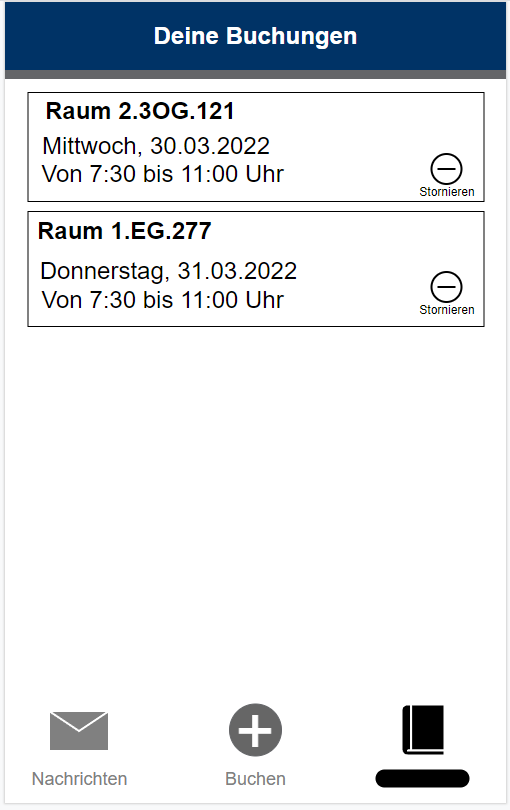
\includegraphics[width=5.5cm]{sketchBuchungen.png}
  \caption{User Interface: Ansicht der getätigten Buchungen}
\end{wrapfigure}

Durch einen Klick auf das Buch in der Funktionsleiste unten, wechselt man in die Übersicht aller getätigten Buchungen.
Die Buchungsübersicht wird in Abbildung 9 dargestellt und wird ebenfalls wieder durch die schwarze Färbung des Symbols in der Funktionsleiste und dem Balken darunter hervorgehoben. \\
\paragraph{}In diesem Fenster werden alle Buchungen als Kacheln angezeigt, welche im System getätigt wurden.
Dabei umfasst jede Kachel den Raum, in dem die Buchung gemacht wurde, das Datum und den Zeitraum der gebucht wurde. \\
\paragraph{}In diesem Fenster lässt sich auch jede getätigte Buchung wieder stornieren durch einen Klick auf das Minus-Symbol.
\\
\\
\\
\\
\newpage
\subsubsection{Nachrichten}

\begin{wrapfigure}{r}{5.5cm}
  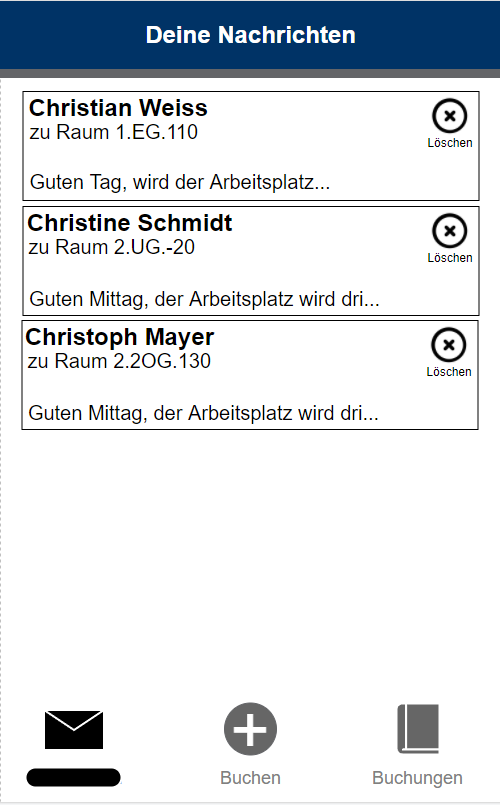
\includegraphics[width=5.5cm]{sketchNachrichten.png}
  \caption{User Interface: Nachrichtenübersicht}
\end{wrapfigure}

Mit einem Klick auf das Briefsymbol, links in der Funktionsleiste, gelangt man zur Nachrichtenübersicht.
Dieses Symbol zeigt auch mit einer kleinen hochgestellten Zahl neben dem Icon an, dass ungelesene Nachrichten eingegangen sind
\paragraph{}In der Nachrichtenübersicht erhält man sämtliche Chats, die man selbst gestartet hat oder an einen persönlich gerichtet sind. 
Denn wie zuvor schon erwähnt, kann man Kollegen eine Nachricht schreiben, wenn diese einen Arbeitsplatz gebucht haben, den man jedoch selbst benötigt. 
Dies geschieht über die Zeitraumeingabe, beim Klicken des "`Benachrichtigen"' Buttons, wenn ein Arbeitsplatz, zur gewünschten Zeit, belegt ist.
\paragraph{} In der Nachrichtenübersicht erhält man, wie bei der Buchungsübersicht, ebenfalls alle offenen Chats als Kacheln aufgelistet. 
Diesmal enhalten die Kacheln den Namen des anderen Chatteilnehmers, den Raum in dem die betroffene Buchung ist und den Textanfang der neusten Nachricht im Chat.
Chatkacheln mit ungelesenen Nachrichten werden zudem noch hervorgehoben.

\paragraph{} Falls sich das betreffende Thema des jeweilgen Chats erledigt hat, kann man den Chat löschen für mehr Übersichtlichkeit in der Nachrichtenübersicht.
Dazu lässt sich jeder Chat löschen, mit einem Klick auf das X-Symbol der jeweiligen Kachel.
Dies löscht den Chat nur persönlich und nicht für den anderen Chatteilnehmer, dieser kann den Chat solange einsehen, bis er ihn auch löscht.

\newpage
\begin{wrapfigure}{r}{5.5cm}
  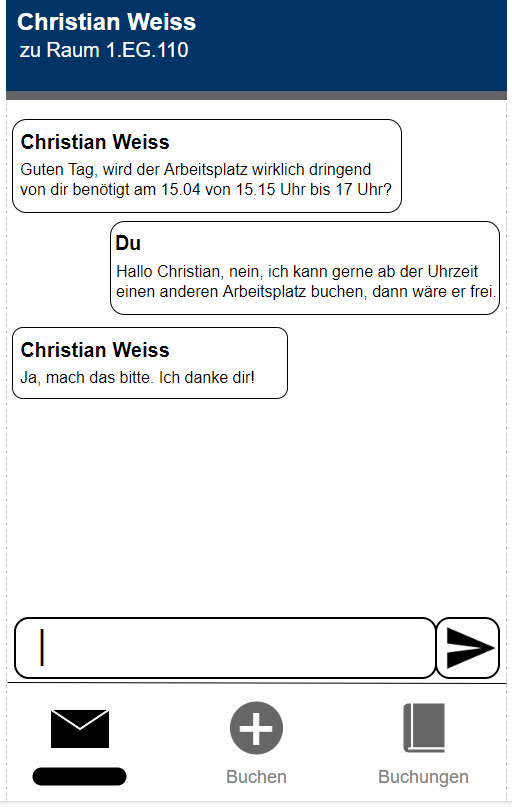
\includegraphics[width=5.5cm]{sketchChat.png}
  \caption{User Interface: Beispielchat}
\end{wrapfigure}

Durch das Anklicken einer Kachel in der Nachrichtenübersicht in Abbildung 10, erhält man den Chat inklusive Chatverlauf.
Der Chat ist in Abbildung 11 dargestellt.

\paragraph{} Im Kopf des Chats sieht man nochmal die gleichen Informationen, wie in der Übersicht, bisauf den Anfang der neusten Nachricht. 
Direkt darunter ist der Chatverlauf.
Eigene Nachrichten sind hierbei nach rechts verschoben und Nachrichten des Gegenüber nach links.

\paragraph{}Überhalb der Funktionsleiste ist noch der Eingabeleiste, welchen man anklickt um eine Nachricht zu verfassen. 
Dieser öffnet schließlich die Texteingabe des Gerätes.
Nach fertigem Verfassen der Nachricht kann man diese abschicken mit dem Symbol rechts neben der Eingabeleiste. 
\\
\\
\\
\\
\\
\\
\subsection{Administrator User Interface}

Nachfolgend wird auf das Interface für Administratoren und Geschäftsführer eingegangen. 
Dies wird genutzt um neue Räume im System zu Registrieren, zu löschen und zu bearbeiten.
Ebenfalls lassen sich dort Nutzergruppen verwalten, die bestimmen, welcher Mitarbeiten in welchem Raum buchen kann. 

\newpage
\subsubsection{Raum-Editor}
Die genannten Aufgaben des Administrator User Interfaces lassen sich in dem Editor, in Abbildung 12, vornehmen.

\begin{figure}[!h]
  \centering
  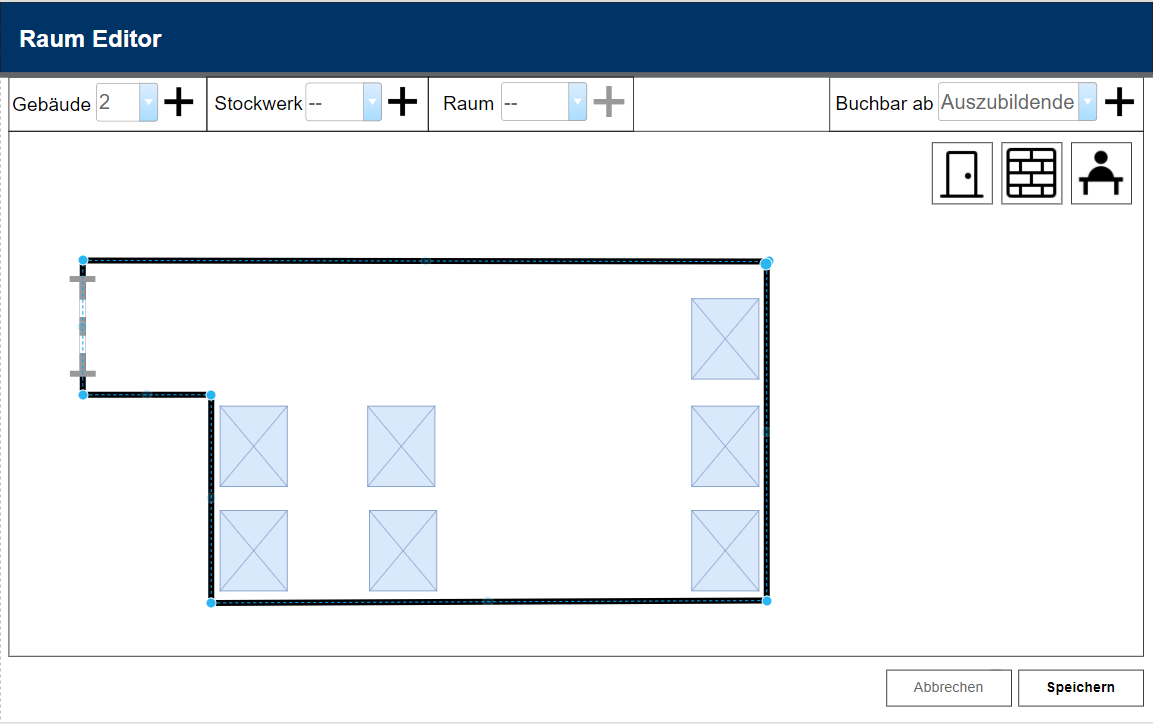
\includegraphics[width=1\textwidth]{sketchEditor.png}
  \caption{User Interface: Raum-Editor}
  \label{fig:sketch_RaumEditor}
\end{figure}

Von oben nach unten durchgehend, werden nachfolgen die Funktionen des Editors erklärt.
\\
Oben links besitzt der Editor Auswahlmöglichkeiten für das Gebäude, die Etage und den Raum.
Ausgewählt wird über Dropdown Menus, welche von links nach rechts ausgewählt werden müssen, wie in der normalen Raumwahl im Buchen Fenster.
Mit einem Rechtsklick auf Einträge im Dropdown Menu lassen sich Räume löschen.
Über das Plus-Symbol rechts neben dem Dropdown Menü kann ein neuer Eintrag jeweils zum System hinzugefügt werden.
Dabei ist es so, dass immer ein Gebäude hinzugefügt werden kann, da dies nicht von vorherigen Auswahlen abhängt. 
Um eine Etage hinzuzufügen, muss ein Gebäude ausgewählt sein, damit die Etage dem ausgewählten Gebäude zugeordnet werden kann.
Zuletzt kann ein Raum hinzugefügt werden, indem ein Gebäude und eine Etage ausgewählt ist.
\\
Bei sämtlichem Hinzufügen erscheint eine Eingabeleiste für den Namen des Eintrags.
Die Eingabe bestätigt man schließlich mit ok und man verwerft sie mit dem X-Symbol.

\paragraph{} Hat man nun einen Raum ausgewählt oder ist soweit, dass man einen neuen erstellt hat, kann man oben rechts die Gruppe auswählen, ab welcher der Raum buchbar ist.
Dies geschieht ebenfalls über ein Dropdown Menu und mit dem +-Symbol erstellt man eine neue Benutzergruppe, die hinzugefügt wird. 

\paragraph{}Mit dem Auswählen oder Erstellen eines Raumes, wird dieser auch unterhalb der oberen Leiste angezeigt. 
In dem Rechteck mit den dünnen schwarzen Linien, lässt sich der Raum interaktiv bearbeiten.
\\
Oben rechts in der Bearbeitungsfläche sind die drei Objekte, die man in den Raum beliebig oft ziehen kann.
Nämlich Türen, Wände und Arbeitsplätze.
Die Visualisierung von Türen, Wänden und Arbeitsplätzen ist in "`3.1.1 Buchen"' beschrieben
\\
Türen lassen sich auf bestehende Wände draufziehen, skalieren und verschieben.
Wände lassen sich einfach in die Bearbeitungsfläche ziehen und wie Polygonlinienzüge anpassen.
Arbeitsplätze werden in den Raum reingezogen und können dort auch noch verschoben und skaliert werden.
Die Elemente in der Bearbeitungsfläche lassen sich generell anklicken und bearbeiten.
Mit der Entf. Taste lässt sich das angeklickte Element auch löschen.

\paragraph{} Untenrechts kann man letztlich die Änderungen an einem Raum komplett verwerfen durch "`Abbrechen"'
oder eben speichern mit "`Speichern"'.
Nach dem Speichern wird ein neuer Raum auch direkt ins System eingefügt.

\subsubsection{Benutzerverwaltung}